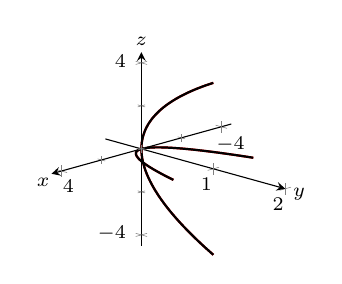
\begin{tikzpicture}[>=stealth]
\begin{axis}%
[width=175pt,tick label style={font=\scriptsize},axis on top,
			axis lines=center,
			view={135}{20},
			name=myplot,
			xtick={-4,4},minor x tick num=3,minor z tick num=3,
			ytick={1,2},
			ztick={-4,4},
			ymin=-0.5,ymax=2,
			xmin=-4.5,xmax=4.5,
			zmin=-4.5, zmax=4.5,
			every axis x label/.style={at={(axis cs:\pgfkeysvalueof{/pgfplots/xmax},0,0)},xshift=-3pt,yshift=-3pt},
				xlabel={\scriptsize $x$},
			every axis y label/.style={at={(axis cs:0,\pgfkeysvalueof{/pgfplots/ymax},0)},xshift=5pt,yshift=-2pt},
				ylabel={\scriptsize $y$},
				every axis z label/.style={at={(axis cs:0,0,\pgfkeysvalueof{/pgfplots/zmax})},xshift=0pt,yshift=4pt},
				zlabel={\scriptsize $z$}
			]

%\addplot3[domain=0:360,smooth,y domain=0:1,surf,%fill=white,
%colormap={mp2}{\colormapplaneone},faceted color=black!40,samples=40,samples y=10,very thin,z buffer=sort] ({2*cos(x)*y},{y^2},{4*y*sin(x)});

\ifthenelse{\boolean{colorprint}}{%
%%% in color
\addplot3[domain=-1:1,,thick,smooth,samples y=0,red,%surf,%fill=white,
samples=30,] ({0},{x^2},{4*x});

\addplot3[domain=-1:1,,thick,smooth,samples y=0,red,%surf,%fill=white,
samples=30,] ({2*x},{x^2},{0});

%%% end in color
}{%
%%% in BW
\addplot3[domain=-1:1,,thick,smooth,samples y=0,black,%surf,%fill=white,
samples=30,] ({0},{x^2},{4*x});

\addplot3[domain=-1:1,,thick,smooth,samples y=0,black,%surf,%fill=white,
samples=30,] ({2*x},{x^2},{0});
%%% end in BW
}

\end{axis}

\end{tikzpicture}












